\begin{paracol}{2}
\begin{leftcolumn}
%\fcolorbox{white}{white}{
%\begin{minipage}[c][0.95\textheight][t]{\linewidth}


%---------------------------------------------------------------------------------------
%	TITLE HEADLINE
%----------------------------------------------------------------------------------------
\vspace{-3pt}
% use this for multiple words like working titles etc.
%\hspace{-0.25\linewidth}\colorbox{bgcol}{\makebox[1.5\linewidth][c]{\hspace{46pt}\HUGE{\textcolor{white}{\uppercase{M.Sc. Jan Küster}} } \textcolor{sectcol}{\rule[-1mm]{1mm}{0.9cm}} \parbox[b]{5cm}{   \large{ \textcolor{white}{{IT Consultant}}}\\
% \large{ \textcolor{white}{{JS Fullstack Engineer}}}}
%}}

% use this for single words, e.g. CV or RESUME etc.
\colorbox{bgcol}{\makebox[\linewidth][c]{\HUGE{\textcolor{white}{\uppercase{Jérémie Libeau}} } \textcolor{sectcol}{\rule[-1mm]{1mm}{0.9cm}} \HUGE{\textcolor{white}{\uppercase{CV}} } }}

%----------------------------------------------------------------------------------------
%	HEADER IMAGE
%----------------------------------------------------------------------------------------


%\hspace{-1.6cm}
%\includegraphics[trim= 0 250 0 270,clip,width=1\linewidth+3.1cm]{myfoto.jpg}	%trimming relative to image size!
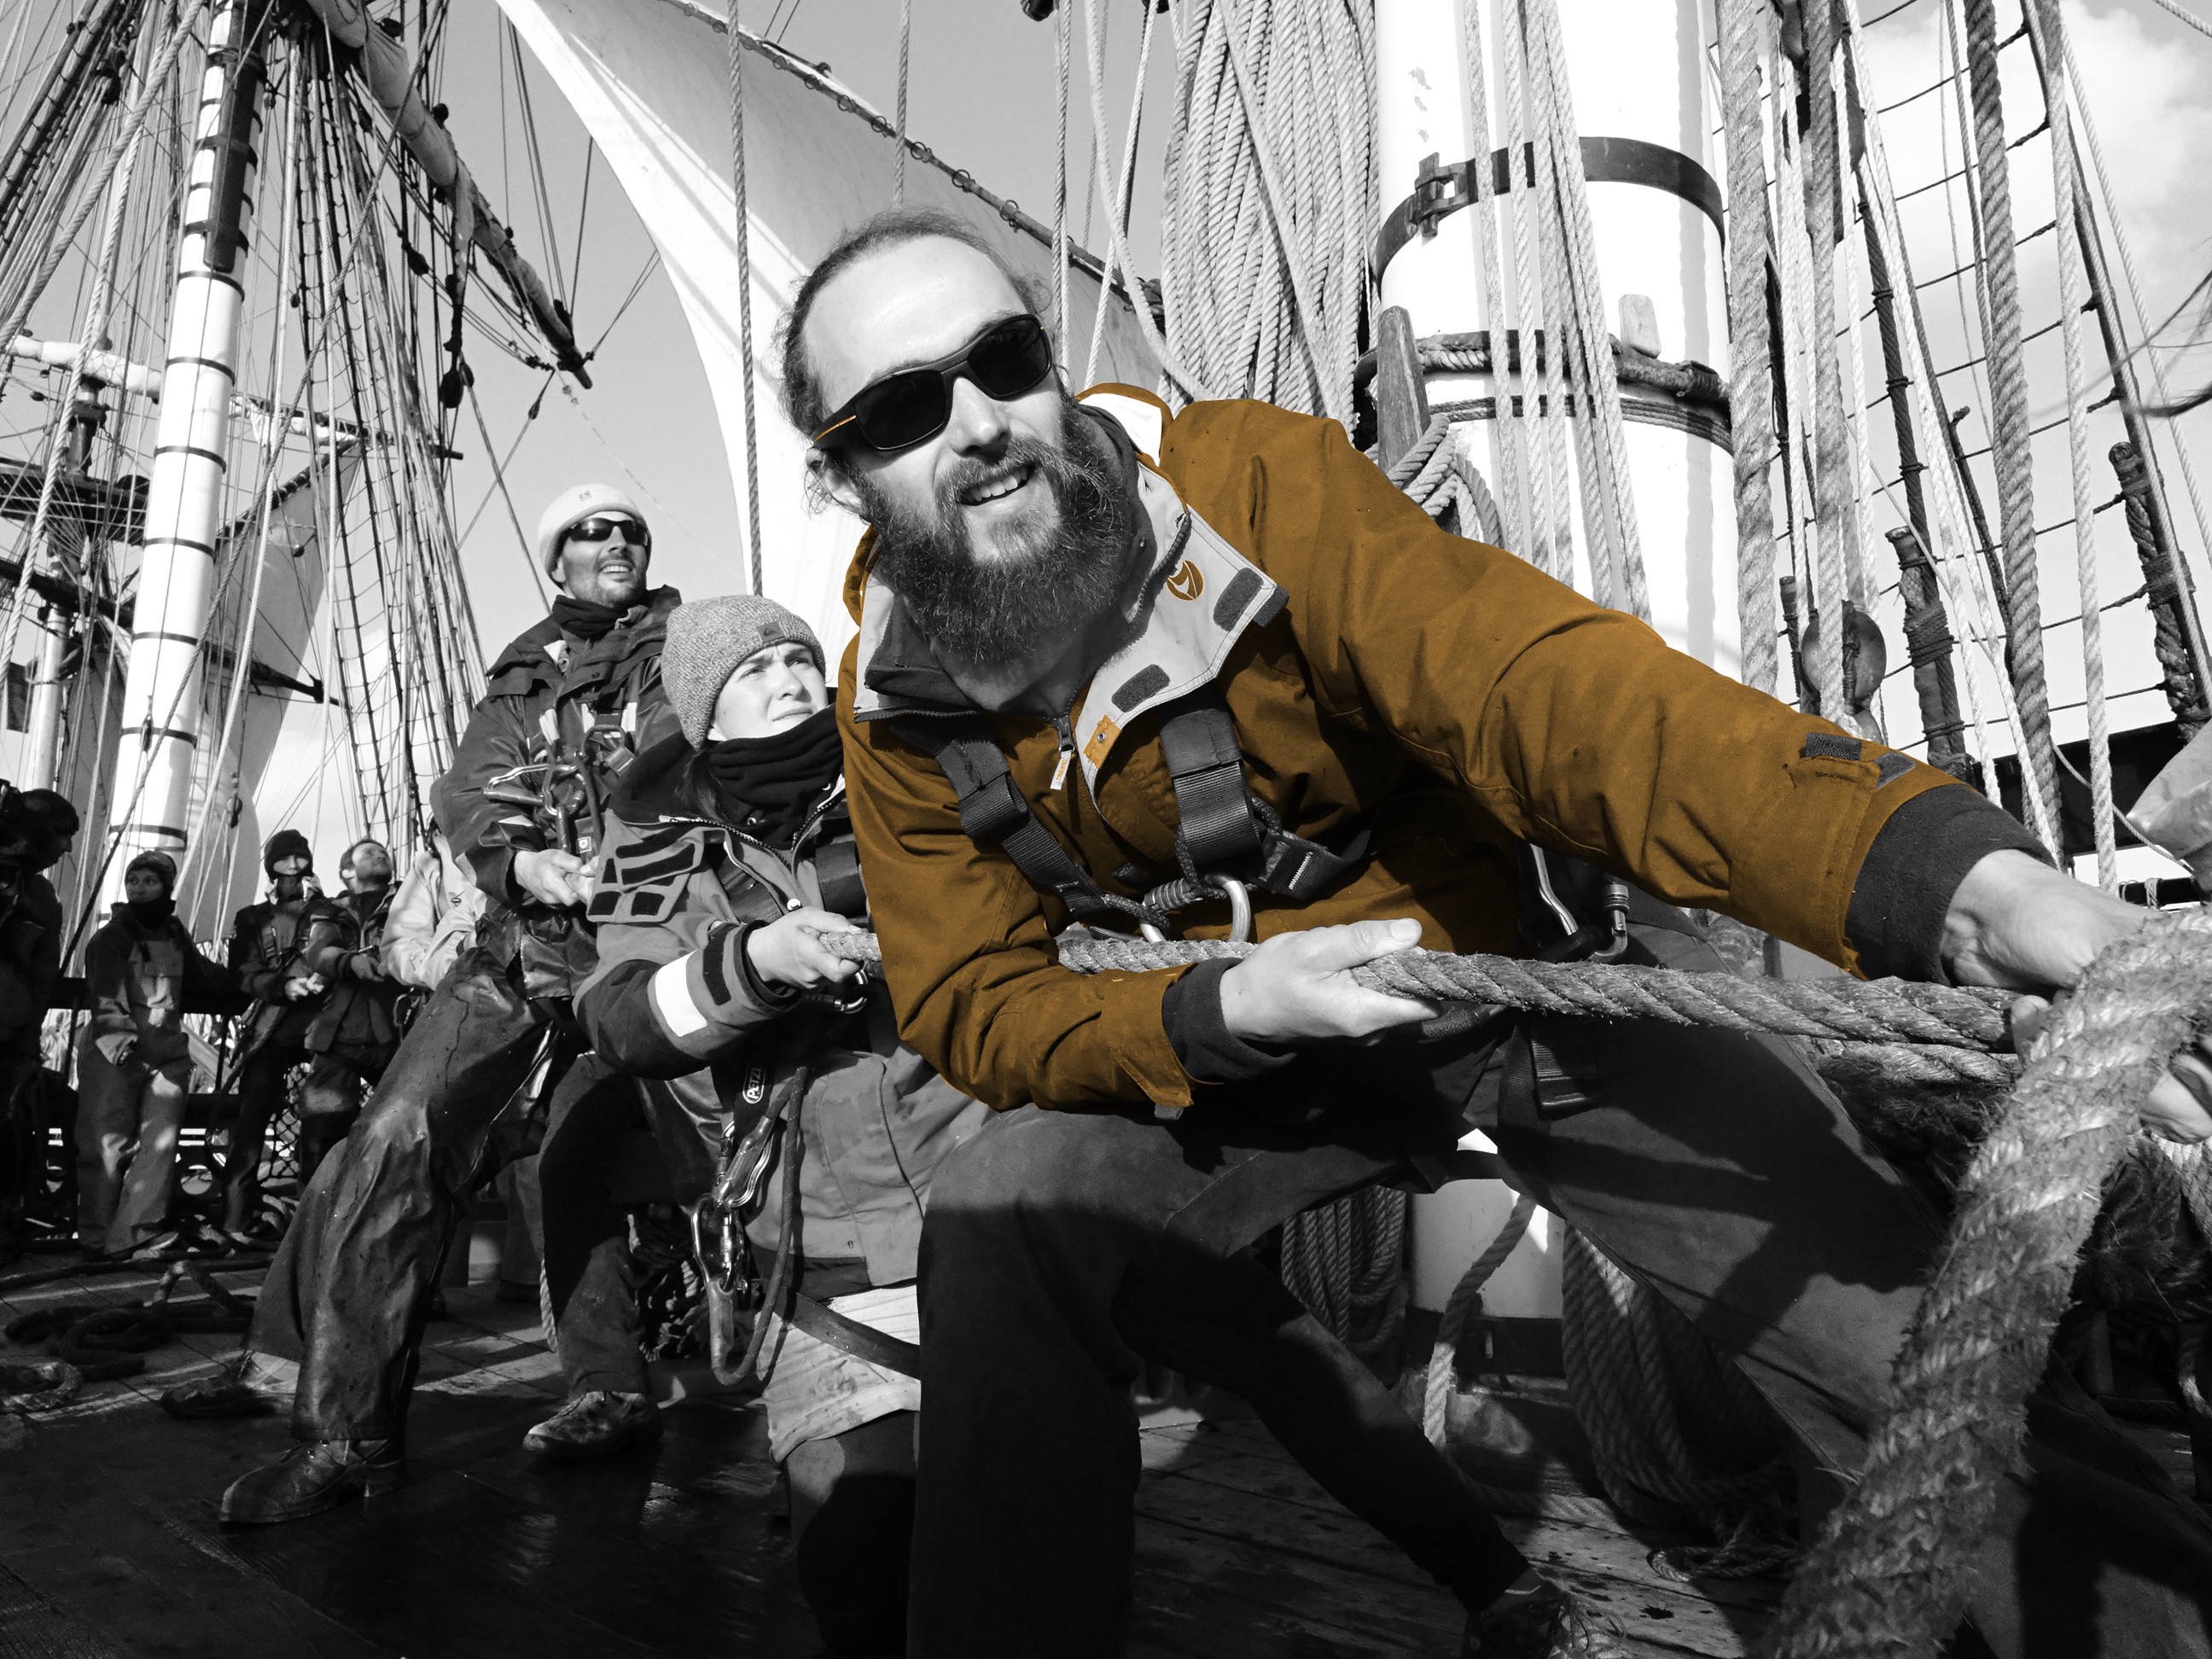
\includegraphics[trim= 100 150 0 40, clip ,width=\linewidth+5px]{images/photo.jpg}	%trimming relative to image size

%---------------------------------------------------------------------------------------
%	SUMMARY
%----------------------------------------------------------------------------------------
\transparent{0.85}%
\vspace{-180pt}
\hspace{0.59\linewidth}
\colorbox{bgcol}{
	\parbox{0.35\linewidth}{
		\transparent{1}%
		\begin{center}
		\tzlbrace{sectcol}\textcolor{white}{Dialoguer | Penser | Créer}\tzrbrace{sectcol}
		\end{center}
	}
}
\vspace{145pt}

%============================================================================%
%
%	CV SECTIONS AND EVENTS (MAIN CONTENT)
%
%============================================================================%

%---------------------------------------------------------------------------------------
%	STATUS
%----------------------------------------------------------------------------------------
\cvsection{Statut}

Développeur fullstack | Tech Lead

\vspace{12pt}

%---------------------------------------------------------------------------------------
%	EDUCATION SECTION
%--------------------------------------------------------------------------------------
\cvsection{Cursus}

\cvevent{2010}{Diplôme d'expert en ingénierie informatique - bac+5}{Epita}{Kremlin-Bicêtre}{
	En alternance à Siemens Mobility à Châtillon}

\cvevent{2007}{DUT Informatique}{IUT de Vannes}{}{
	Option Génie Logiciel}

\cvevent{2005}{Baccalauréat Scientifique - mention Assez Bien}{Lycée Chevrollier}{Angers}{
	Spécialisation Sciences de l'Ingénieur}

\vspace{12pt}

%---------------------------------------------------------------------------------------
%	EXPERIENCE
%----------------------------------------------------------------------------------------
\cvsection{Expériences}

\cvevent{2026/03}{Développeur fullstack - freelance}{Astrolabe}{Rennes \emph{en remote}}{
	Développement fullstack \emph{PHP} et \emph{React}.
}

\cvevent{2023/03 - 2025/12}{Tech lead}{EGERIE}{Toulon \emph{en remote}}{
    Développement backend \emph{PHP}{,} framework \emph{Silex} et \emph{Symfony},
	Développement \emph{React},
    Coordination du \emph{chapter back},
    Mise en place et suivi des bonnes pratiques de développement liées à la qualité du code \emph{clean code}{,} \emph{SOLID},
    Design d'une architecture \emph{Hexagonal} avec \emph{API Platform},
    Rédaction d'\emph{ADR} discutée en \emph{guild},
    Accompagnement technique des développeurs,
    Développement de tests unitaires et fonctionnels via \emph{PHPUnit}
}

\cvevent{2018/01 - 2023/03}{Développeur fullstack / DevOps}{Symetri}{Rennes}{
	Backend \emph{PHP}{,} framework \emph{Symfony} et \emph{Zend}{,} base de données \emph{MSSql},
	Frontend web \emph{JS} et framework \emph{Angular},
	Administration de la plateforme de production cloud OBS,
	Développement de tests unitaires et fonctionnels via \emph{PHPUnit},
	Mise en place d'une plateforme d'intégration et de déploiement continu \emph{Jenkins} puis \emph{Gitlab},
	Dockerisation des applications et mise en place d'une infrastructure \emph{Kubernetes},
	Participation à la coordination projet \emph{SCRUM}}

\cvevent{2014/05 - 2017/12}{Développeur fullstack}{Avenue du Web}{Rennes}{
	Backend \emph{PHP} et framework \emph{Symfony 2}{,} base de données \emph{MySQL},
	Développement d'un système de commentaire live web{,} basé sur websocket,
	Frontend JS,
	Administration des outils de développement,
	Développement de tests unitaires et fonctionnels via \emph{PHPUnit},
	Mise en place d'une plateforme de tests automatiques \emph{Jenkins},
	Participation à la coordination projet \emph{SCRUM}}

\cvevent{2013/06 - 2014/03}{Développeur fullstack}{Outscale}{Saint-Cloud}{
	Développement avec \emph{PHP} \emph{Silex} et \emph{RubyOnRails},
	Développement et intégration de logiciels de reporting et de facturation,
	Documentation technique,
	Participation à la coordination projet \emph{SCRUM}}

\cvevent{2011/08 - 2013/02}{Data Manager}{Ubisoft}{Montreuil}{
	Support technique sur les différentes consoles du marché et à venir,
	Tests de qualité sur les jeux en développement,
	Gestion de l'archivage des différentes versions des jeux,
	Gestion de l'espace de partage documentaire,
	Rédaction de documentation}

\cvevent{2007/10 - 2010/10}{Administrateur Systèmes Unix/Linux}{Siemens Mobility}{Châtillon}{
	Apprentissage de 3 ans dans le cadre du diplôme d'ingénieur expertise informatique,
	Réponse aux besoins utilisateur,
	Étude et mise en place d'un nouveau parc de machines Suse Linux,
	Supervision du data center via cacti et nagios,
	Développement d'outils d'aide à la production}

\vspace{12pt}

%---------------------------------------------------------------------------------------
%	EDUCATION SECTION
%--------------------------------------------------------------------------------------
\cvsection{Formations}

\cvevent{2014/06}{Développement web avec Symfony2}{SensioLabs}{}{
	4 jours,
	Maîtrise du framework Symfony 2}

\vspace{12pt}

\cvsection{Engagements associatifs}

\cvevent{2016 - 2018}{Membre du CA}{Association Grifon}{}{
	Grifon a pour but la promotion{,} l'utilisation et le développement d'Internet localement,
	Participe aux discutions avec les collectivités locales pour le projet d'utilisation du réseau en fibre optique de la ville et pour le projet de collecte ADSL via Rennes Métropole Télécom,
	\href{https://grifon.fr/}{grifon.fr}}

\cvevent{2016 - 2018}{Membre actif}{Fédération FDN}{}{
	La fédération FDN regroupe des Fournisseurs d'Accès à Internet associatifs se reconnaissant dans des valeurs communes : bénévolat{,} solidarité{,} fonctionnement démocratique et à but non lucratif; défense et promotion de la neutralité du Net,
	\href{https://www.ffdn.org/}{ffdn.org}}

\cvevent{2018 et 2019}{Gabier}{Association Hermione-La Fayette}{}{
	Gabier sur L'Hermione sur les voyages 2018 et 2019,
	\href{https://fregate-hermione.com/}{fregate-hermione.com}}


\end{leftcolumn}

\begin{rightcolumn}

\begin{metasection}{Contact}

    \iconnewtext{F3C5}{12}{Trédarzec, Bretagne}{white}\\[6pt]
	\icontel{Mobile}{12}{0687463241}{06 87 46 32 41}{white}\\[6pt]
    \iconnewemail{F1D8}{12}{job@jeremielibeau.fr}{job@jeremielibeau.fr}{white}\\[6pt]
    \iconhref{Globe}{12}{https://jeremielibeau.fr/}{https://jeremielibeau.fr/}{white}\\[6pt]
    \iconhref{Github}{12}{https://github.com/loconox/}{https://github.com/loconox/}{white}\\[6pt]

\end{metasection}

%----------------------------------------------------------------------------------------
%	META SECTION
%----------------------------------------------------------------------------------------

\begin{metasection}{Domaines}

\icontext{Code}{12}{Développement backend}{white}\\
\icon{Star}{12}{complcol}\icon{Star}{12}{complcol}\icon{Star}{12}{complcol}\icon{Star}{12}{complcol}\icon{Star}{12}{complcol}\icon{Star}{12}{complcol}\icon{Star}{12}{complcol}\icon{Star}{12}{complcol}\icon{Star}{12}{complcol}\icon{Star}{12}{complcol}\\[6pt]

\icontext{HexagonNodes}{12}{Architecture logiciel}{white}\\
\icon{Star}{12}{complcol}\icon{Star}{12}{complcol}\icon{Star}{12}{complcol}\icon{Star}{12}{complcol}\icon{Star}{12}{complcol}\icon{Star}{12}{complcol}\icon{Star}{12}{complcol}\icon{Star}{12}{complcol}\icon{Star}{12}{white}\icon{Star}{12}{white}\\[6pt]

\icontext{Lightbulb}{12}{Lead technique}{white}\\
\icon{Star}{12}{complcol}\icon{Star}{12}{complcol}\icon{Star}{12}{complcol}\icon{Star}{12}{complcol}\icon{Star}{12}{complcol}\icon{Star}{12}{complcol}\icon{Star}{12}{complcol}\icon{Star}{12}{white}\icon{Star}{12}{white}\icon{Star}{12}{white}\\[6pt]

\icontext{Docker}{12}{Devops}{white}\\
\icon{Star}{12}{complcol}\icon{Star}{12}{complcol}\icon{Star}{12}{complcol}\icon{Star}{12}{complcol}\icon{Star}{12}{complcol}\icon{Star}{12}{complcol}\icon{Star}{12}{white}\icon{Star}{12}{white}\icon{Star}{12}{white}\icon{Star}{12}{white}\\[6pt]

\end{metasection}

\begin{metasection}{\technologiesTitle}

\textcolor{white}{
	\icontext{Php}{12}{PHP}{white}
	\icontext{Symfony}{12}{Symfony}{white} \\[6pt]
	\icontext{Code}{12}{Zend}{white}
	\icontext{Js}{12}{Javascript}{white} \\[6pt]
	\iconcustomtext{images/angular.png}{12}{Angular}{white}
    \icontext{React}{12}{React}{white} \\[6pt]
	\icontext{Docker}{12}{Docker}{white}
	\icontext{Linux}{12}{Linux}{white} \\[6pt]
	\icontext{Cloud}{12}{Cloud}{white}
}
\end{metasection}


\begin{metasection}{\toolsTitle}

\textcolor{white}{
	\iconcustomtext{images/PhpStorm.png}{12}{PhpStorm}{white}
	\icontext{Openai}{12}{IA}{white}\\[6pt]
	\icontext{Terminal}{12}{Terminal}{white} \icontext{Gitlab}{12}{Gitlab}{white} \\[6pt]
    	\icontext{Jira}{12}{Jira}{white}
}
\end{metasection}



\begin{metasection}{OS}

    \textcolor{white}{\LARGE{\icon{Linux}{24}{white} \icon{Apple}{24}{white}  \icon{Windows}{24}{white}}}

\end{metasection}


\newpage

\begin{metasection}{Activities}

	\textcolor{white}{\LARGE{\icon{BattleNet}{24}{white} \icon{Anchor}{24}{white}  \iconnew{F86B}{24}{white}}}

\end{metasection}

\begin{metasection}{Langues}

	\textcolor{white}{Français}\\
	\icon{Star}{12}{complcol}\icon{Star}{12}{complcol}\icon{Star}{12}{complcol}\icon{Star}{12}{complcol}\icon{Star}{12}{complcol}\icon{Star}{12}{complcol}\icon{Star}{12}{complcol}\icon{Star}{12}{complcol}\icon{Star}{12}{complcol}\icon{Star}{12}{complcol}\\[6pt]

	\textcolor{white}{Anglais}\\
	\icon{Star}{12}{complcol}\icon{Star}{12}{complcol}\icon{Star}{12}{complcol}\icon{Star}{12}{complcol}\icon{Star}{12}{complcol}\icon{Star}{12}{complcol}\icon{Star}{12}{complcol}\icon{Star}{12}{white}\icon{Star}{12}{white}\icon{Star}{12}{white}\\[6pt]

	\textcolor{white}{Espagnol}\\
	\icon{Star}{12}{complcol}\icon{Star}{12}{complcol}\icon{Star}{12}{white}\icon{Star}{12}{white}\icon{Star}{12}{white}\icon{Star}{12}{white}\icon{Star}{12}{white}\icon{Star}{12}{white}\icon{Star}{12}{white}\icon{Star}{12}{white}\\[6pt]

\end{metasection}


%\end{minipage}}


%============================================================================%
%
%
%
%	DOCUMENT END
%
%
%
%============================================================================%
\end{rightcolumn}
\end{paracol}

%-------------------------------------------------------------------------------------------------
%	ARTIFICIAL FOOTER (fancy footer cannot exceed linewidth)
%--------------------------------------------------------------------------------------------------

%\null
%\vspace*{\fill}
%\hspace{-0.25\linewidth}\colorbox{bgcol}{\makebox[1.5\linewidth][c]{\mystrut \small \textcolor{white}{Coypright 2018 jkuester@uni-bremen.de} $\cdot$ \textcolor{white}{licensed under MIT license}}}\\[-6pt]
